\section{Thu thập, đánh giá MBTI từ người dùng}
Để giúp người dùng có thể hiểu được nhóm tính cách MBTI của mình, nhóm sử dụng bộ câu hỏi tiêu chuẩn bao gồm 70 câu. Bộ câu hỏi này được nhiều trang web lớn của Việt Nam tin dùng như nền tảng lựa chọn nghề nghiệp hàng đầu Việt Nam - TopCV hay Đại học Ngân hàng Thành phố Hồ Chí Minh. Nhóm chúng em sử dụng bản được biên dịch và công bố công khai của công ty TNHH THANH BÌNH PSY - một công ty tư vấn tâm lý có tiếng trên địa bàn thành phố Hồ Chí Minh.

Bộ câu hỏi bao gồm:
\begin{multicols}{2}
\noindent \textbf{Câu 1:} Tại một buổi tiệc, bạn sẽ: \\
a. Giao tiếp với nhiều người, kể cả người lạ \\
b. Chỉ giao tiếp với với một số ít người mà bạn đã quen \\
\textbf{Câu 2:} Bạn thấy mình là người nghiêng về kiểu nào nhiều hơn? \\
a. Thực tế \\
b. Sáng tạo \\
\textbf{Câu 3:} Bạn nghĩ tình huống nào tồi tể hơn? \\
a. Đầu óc của bạn cứ “bay bổng" trên mây \\
b. Cuộc sống của bạn thật nhàm chán và không bao giờ thay đổi \\
\textbf{Câu 4:} Bạn sẽ bị ấn tượng hơn với \\
a. Các nguyên tắc \\
b. Những cảm xúc \\
\textbf{Câu 5:} Khi quyết định việc gì đó, bạn thường hay dựa vào: \\
a. Sự thuyết phục \\
b. Sự đồng cảm \\
\textbf{Câu 6:} Bạn thích làm việc theo kiểu nào nhiều hơn? \\
a. Theo đúng thời hạn \\
b. Tùy hứng \\
\textbf{Câu 7:} Bạn có khuynh hướng đưa ra các lựa chọn \\
a. Rất cẩn thận \\
b. Phần nào theo cảm nhận \\
\textbf{Câu 8:} Tại các bữa tiệc, bạn thường: \\
a. Ở lại tới cùng và cảm thấy càng lúc càng hào hứng \\
b. Ra về sớm vì cảm thấy mệt mỏi dần \\
\textbf{Câu 9:} Kiểu người nào sẽ thu hút bạn hơn? \\
a. Người thực tế và có lý lẽ \\
b. Người giàu trí tưởng tượng \\
\textbf{Câu 10:} Điều nào khiến bạn thấy thích thú hơn? \\
a. Những điều thực tế \\
b. Những ý tưởng khả thi \\
\textbf{Câu 11:} Khi đánh giá hoặc phán xét người khác, bạn thường hay dựa vào điều gì? \\
a. Luật lệ và nguyên tắc \\
b. Hoàn cảnh \\
\textbf{Câu 12:} Khi tiếp cận, tiếp xúc người khác, bạn nghiêng về hướng nào hơn? \\
a. Tiếp cận theo hướng khách quan \\
b. Tiếp cận theo hướng sử dụng trải nghiệm cá nhân \\
\textbf{Câu 13:} Phong cách của bạn nghiêng về hướng nào hơn? \\
a. Đúng giờ, nghiêm túc \\
b. Nhàn nhã, thoải mái \\
\textbf{Câu 14:} Bạn cảm thấy không thoải mái khi có những việc: \\
a. Chưa hoàn thiện \\
b. Đã quá hoàn thiện \\
\textbf{Câu 15:} Trong các mối quan hệ xã hội, bạn thường \\
a. Luôn nắm bắt kịp thời thông tin về các vấn đề của mọi người \\
b. Thường biết thông tin sau những người khác \\
\textbf{Câu 16:} Với các công việc thông thường, bạn nghiêng về cách: \\
a. Làm theo cách thông thường \\
b. Làm theo cách của riêng mình \\
\textbf{Câu 17:} Các nhà văn nên: \\
a. Viết những gì họ nghĩ và chân thật với những gì mình viết \\
b. Diễn đạt sự việc bằng cách so sánh hay liên tưởng \\
\textbf{Câu 18:} Điều gì lôi cuốn bạn hơn? \\
a. Tính nhất quán của tư duy, suy nghĩ \\
b. Sự hòa hợp trong các mối quan hệ của con người \\
\textbf{Câu 19:} Bạn cảm thấy thoải mái hơn khi đưa ra: \\
a. Những đánh giá, nhận xét một cách logic \\
b. Những đánh giá, nhận xét một cách có ý nghĩa \\
\textbf{Câu 20:} Bạn thích những điều: \\
a. Đã được sắp xếp, quyết định trước \\
b. Chưa xác định, chưa được quyết định \\
\textbf{Câu 21:} Bạn tự thấy mình: \\
a. Nghiêm túc, quyết đoán \\
b. Dễ gần, thoải mái \\
\textbf{Câu 22:} Khi nói chuyện điện thoại, bạn: \\
a. Cứ gọi bình thường \\
b. Chuẩn bị trước những điều sẽ nói \\
\textbf{Câu 23:} Những sự kiện trong thực tế \\
a. Bản thân nó giải thích cho chính nó \\
b. Nó là bằng chứng giải thích cho các quy tắc, quy luật \\
\textbf{Câu 24:} Những người có tầm nhìn xa/người lo xa. \\
a. Thường gây khó chịu cho người khác \\
b. Khá thú vị \\
\textbf{Câu 25:} Bạn thường là người \\
a. Cái đầu lạnh \\
b. Trái tim nóng \\
\textbf{Câu 26:} Điều nào thì tồi tệ hơn? \\
a. Không công bằng \\
b. Tàn nhẫn \\
\textbf{Câu 27:} Các sự kiện nên xảy ra theo hướng: \\
a. Được lựa chọn và cân nhắc kỹ lưỡng \\
b. Ngẫu nhiên và tự nhiên \\
\textbf{Câu 28:} Bạn cảm thấy thoải mái hơn khi \\
a. Đã mua một thứ gì đó \\
b. Đang lựa chọn để mua \\
\textbf{Câu 29:} Trong công ty, bạn là người: \\
a. Khởi xướng các câu chuyện \\
b. Đợi người khác bắt chuyện với mình \\
\textbf{Câu 30:} Đối với những quy ước, quy tắc thông thường trong xã hội, bạn: \\
a. Ít khi nghi ngờ những điều này \\
b. Thường xem xét lại tính đúng đắn của những điều đó \\
\textbf{Câu 31:} Trẻ em thường: \\
a. Chưa cố gắng đủ \\
b. Chưa vui chơi đủ \\
\textbf{Câu 32:} Khi đưa ra các quyết định, bạn sẽ thấy thoải mái hơn với \\
a. Các tiêu chuẩn \\
b. Cảm xúc, cảm nhận \\
\textbf{Câu 33:} Bạn nghiêng về tính cách nào hơn? \\
a. Cứng rắn \\
b. Nhẹ nhàng \\
\textbf{Câu 34:} Theo bạn, khả năng nào đáng khâm phục hơn? \\
a. Khả năng tổ chức và làm việc có phương pháp \\
b. Khả năng thích ứng và xoay xở trước mọi tình huống \\
\textbf{Câu 35:} Bạn đề cao tố chất nào hơn? \\
a. Sự chắc chắn \\
b. Sự cởi mở \\
\textbf{Câu 36:} Khi phải tương tác với người khác ở các tình huống và vấn đề mới lạ, không thường gặp, bạn thường: \\
a. Thấy phấn chấn và hào hứng \\
b. Cảm thấy mệt mỏi \\
\textbf{Câu 37:} Thường thì bạn là: \\
a. Người thực tế \\
b. Người có khả năng tưởng tượng phong phú \\
\textbf{Câu 38:} Bạn thường có xu hướng: \\
a. Xem người khác có thể làm được việc gì hữu ích \\
b. Xem người khác sẽ nghĩ và cảm nhận như thế nào \\
\textbf{Câu 39:} Bạn cảm thấy thoải mái hơn khi: \\
a. Thảo luận một vấn đề kỹ lưỡng, triệt để \\
b. Đạt được thỏa thuận, sự nhất trí về vấn đề \\
\textbf{Câu 40:} Cái đầu hay trái tim chi phối bạn nhiều hơn \\
a. Cái đầu \\
b. Trái tim \\
\textbf{Câu 41:} Bạn cảm thấy thoải mái hơn khi làm các công việc theo dạng \\
a. Được giao trọn gói, làm xong hết rồi bàn giao \\
b. Công việc làm hàng ngày, theo lịch \\
\textbf{Câu 42:} Bạn có xu hướng tìm kiếm những điều: \\
a. Theo trật tự, thứ tự \\
b. Ngẫu nhiên \\
\textbf{Câu 43:} Bạn thích kiểu nào hơn? \\
a. Nhiều bạn bè ở mức độ xã giao \\
b. Một vài người bạn thân \\
\textbf{Câu 44:} Bạn thường dựa vào: \\
a. Sự kiện, thông tin thực tế \\
b. Nguyên lý, nguyên tắc \\
\textbf{Câu 45:} Bạn hứng thú với việc gì hơn? \\
a. Sản xuất và phân phối \\
b. Thiết kế và nghiên cứu \\
\textbf{Câu 46:} Lời khen nào giá trị hơn? \\
a. “Đó là một người có suy nghĩ rất logic” \\
b. “Đó là một người rất tình cảm, tinh tế” \\
\textbf{Câu 47:} Bạn thích mình có tố chất nào hơn? \\
a. Kiên định, vững vàng \\
b. Toàn tâm, cống hiến \\
\textbf{Câu 48:} Bạn thường thích điều nào hơn? \\
a. Một tuyên bố cuối cùng, không thay đổi \\
b. Một tuyên bố dự kiến, ban đầu \\
\textbf{Câu 49:} Bạn thấy thoải mái hơn vào lúc: \\
a. Trước khi đưa ra quyết định \\
b. Sau khi đưa ra quyết định \\
\textbf{Câu 50:} Bạn có thấy mình: \\
a. Dễ dàng bắt chuyện và kéo dài cuộc trò chuyện với người mới gặp \\
b. Khó mà trò chuyện nhiều với những người mới quen \\
\textbf{Câu 51:} Bạn có xu hướng tin tưởng vào: \\
a. Kinh nghiệm của mình \\
b. Linh cảm của mình \\
\textbf{Câu 52:} Bạn cho rằng mình thuộc tuýp người nào hơn? \\
a. Người thực tế \\
b. Người khôn khéo \\
\textbf{Câu 53:} Theo bạn ai là người đáng được khen ngợi hơn? \\
a. Một người giàu lý trí \\
b. Một người giàu cảm xúc \\
\textbf{Câu 54:} Bạn có xu hướng hành xử: \\
a. Công bằng, vô tư \\
b. Thông cảm, đồng cảm \\
\textbf{Câu 55:} Bạn thích: \\
a. Đảm bảo rằng mọi việc được chuẩn bị, thu xếp sẵn sàng \\
b. Để mọi việc diễn ra tự nhiên \\
\textbf{Câu 56:} Trong các mối quan hệ thì mọi việc: \\
a. Có thể thảo luận để giải quyết được \\
b. Diễn ra ngẫu nhiên và tùy theo điều kiện hoàn cảnh \\
\textbf{Câu 57:} Khi chuông điện thoại reo, bạn sẽ: \\
a. Là người đầu tiên nhấc máy \\
b. Hy vọng có người khác sẽ nhấc máy \\
\textbf{Câu 58:} Bạn đánh giá cao điều gì trong mình hơn: \\
a. Nhận thức tốt về các yếu tố thực tế \\
b. Có trí tưởng tượng phong phú, rực rỡ \\
\textbf{Câu 59:} Bạn sẽ chú tâm hơn đến: \\
a. Các nguyên tắc, nguyên lý cơ bản \\
b. Các ngụ ý, hàm ý, ẩn ý \\
\textbf{Câu 60:} Điều gì có vẻ sẽ là một lỗi lớn hơn? \\
a. Quá nồng nhiệt, thiết tha \\
b. Quá khách quan, thờ ơ \\
\textbf{Câu 61:} Về cơ bản, bạn sẽ đánh giá mình là người thế nào? \\
a. Thiết thực, ít bị chi phối bởi tình cảm \\
b. Từ tâm, đa cảm \\
\textbf{Câu 62:} Tình huống nào sẽ lôi cuốn bạn hơn? \\
a. Tình huống rõ ràng, có kế hoạch \\
b. Tình huống không xác định, không có kế hoạch \\
\textbf{Câu 63:} Bạn là người có xu hướng nào hơn? \\
a. Theo thói quen \\
b. Hay thay đổi \\
\textbf{Câu 64:} Bạn có xu hướng nào hơn? \\
a. Là người dễ tiếp cận \\
b. Ở mức độ nào đó là người kín đáo \\
\textbf{Câu 65:} Khi viết, bạn thích: \\
a. Viết theo hướng văn chương hơn \\
b. Viết theo số liệu, dữ liệu hơn \\
\textbf{Câu 66:} Đối với bạn, điều gì khó thực hiện hơn? \\
a. Hiểu và chia sẻ với người khác \\
b. Điều khiển người khác \\
\textbf{Câu 67:} Bạn mong ước mình sẽ có thêm nhiều điều gì? \\
a. Lí trí và khả năng nhận xét rõ ràng \\
b. Tình thương, lòng trắc ẩn sâu sắc \\
\textbf{Câu 68:} Điều gì sẽ là lỗi lớn hơn? \\
a. Hành động bừa bãi, không cân nhắc \\
b. Hành động chỉ trích, phê phán \\
\textbf{Câu 69:} Bạn sẽ thích sự kiện nào hơn? \\
a. Sự kiện có lên kế hoạch trước \\
b. Sự kiện không có kế hoạch trước \\
\textbf{Câu 70:} Bạn thường có hành động: \\
a. Cân nhắc thận trọng \\
b. Tự nhiên, tự phát \\
\end{multicols}

Bộ 70 câu hỏi này được sắp xếp theo thứ tự xác định, sau khi người dùng trả lời xong tiến hành tính toán để phân loại tính cách cho người dùng theo bảng sau.
\begin{figure}[H]
    \centering
    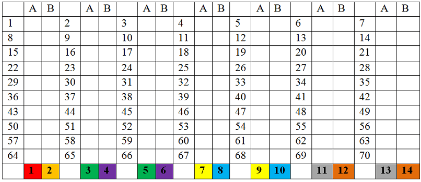
\includegraphics[width=0.8\linewidth]{images/chap3/MBTItable.png}
    \vspace{0.5cm}
    \caption{Bảng phân loại tính cách MBTI}
\end{figure}

\begin{itemize}
    \setlength\itemsep{0em}
    \item E (Hướng ngoại) = Kết quả cột 1
    \item I (Hướng nội) = Kết quả cột 2
    \item S (Giác quan)  = Kết quả cột 3 + 5
    \item N (Trực giác) = Kết quả cột 4 +6
    \item T (Lý trí) = Kết quả cột 7 + 9
    \item F (Cảm xúc) = Kết quả 8 +10
    \item J (Nguyên tắc)  = Kết quả cột 11 + 13
    \item P (Linh hoạt) = Kết quả cột 12 + 14
\end{itemize}

Kết quả được phân tích từ cột có kết quả cao hơn trong mỗi cặp E/I,S/N,T/F, J/P. Từ đó người dùng có thể xác định được loại tính cách phù hợp với bản thân mình